\nolinenumbers

\renewcommand{\thefigure}{\thesection.\arabic{figure}}
\renewcommand{\thetable}{\thesection.\arabic{table}}


\section{Transition Rates}\label{sec:transition_rates}

\subsection{Migration}\label{subsec:migration}

\subsubsection{Default State Space}\label{subsubsec:migration_default}
Let each state be described by $\mathbf{e}=(d_1, \ldots, d_m)$, where $d_i$ is the number of lineages in deme $i$, and $m$ is the number of demes.
Migration events are not allowed to occur concurrently with coalescence or recombination events, and only one lineage can migrate at a time.
We have
\begin{align*}
    s^d_{\phi(\mathbf{e}_1),\phi(\mathbf{e}_2)} =
    \begin{cases}
        m_{ij} \cdot n_i & \text{if }
        \begin{aligned}[t]
            & \mathbf{e}_1=(a_1,\dots,a_n), \\
            & \mathbf{e}_2=(a_1,\dots,a_i-1,\dots,a_j+1,\dots,a_{n}), \\
            & a_i \geq 1,
        \end{aligned} \\
        0 & \text{otherwise,}
    \end{cases}
\end{align*}
where $m_{ij}$ is the migration rate from deme $i$ to deme $j$ backwards in time, and $n_i$ is the number of lineages in deme $i$ prior to the migration event.

\subsubsection{Block-counting State Space}\label{subsubsec:migration_block_counting}
Let each state be described by $e=(\mathbf{d}_1, \ldots, \mathbf{d}_m)$, where $\mathbf{d}_i=(a_{i1}, \ldots, a_{in})$ are the lineage block counts in deme $i$, and $n$ is the initial number of lineages.
We have
\begin{align*}
    s^b_{\phi(\mathbf{e}_1),\phi(\mathbf{e}_2)} =
    \begin{cases}
        m_{ij} \cdot n_{ij} & \text{if }
        \begin{aligned}[t]
            & \mathbf{e}_1=(\mathbf{d}_1,\dots,\mathbf{d}_n), \\
            & \begin{aligned}[t]
                  \mathbf{e}_2 &= ( \\
                  & \mathbf{d}_1, \dots, \\
                  & (a_{i1},\dots,a_{ik}-1,\dots,a_{in}), \dots, \\
                  & (a_{j1},\dots,a_{jl}+1,\dots,a_{jn}), \dots, \\
                  & \mathbf{d}_n \\
            \end{aligned} \\
            & ), \\
            & a_{ik} \geq 1,
        \end{aligned} \\
        0 & \text{otherwise,}
    \end{cases}
\end{align*}
where $n_{ij}$ is the number of lineages in block $j$ of deme $i$ prior to the migration event.
We have one absorbing state for each deme in which the final coalescence event can take place.
When modeling more than one locus, we additionally need to make sure that migration events on modify the lineage block counts consistently across linked loci.

\begin{figure}[H]
    \centering
    \includegraphics[width=\textwidth]{figures/migration_two_lineages_default}
    \caption{
        Transition rates for migration in a two-deme model with two lineages using the default state space.
        Each note represents a state, and each edge a transition.
        States are described by a 2-tuple which respresent the number of lineages and linked lineages, respectively.
        All migration rates and population sizes are 1.
        Green nodes indicate the initial states, and red nodes the absorbing states.
    }
    \label{fig:migration_two_lineages_default}
\end{figure}

%Each state is parameterized by a 3-dimensional array $e_{ijk}$.
%For $i = 0$, $j$ is the deme index and $k$ is the lineage block index of the number of lineages in each deme and lineage block.
%For $i = 1$, $j$ is the deme index and $k$ is the lineage block index of the number of linked lineages in each deme and lineage block.
%For the default state space, there is only one lineage block holding all lineages.
%In alternative terminology, the two elements along the first dimension of $\mathbf{e}$ correspond to the number of lineages and linked lineages, respectively.
%The second dimension to the demes and the third dimension to lineage blocks.
%For example, $[[[1] [1]], [[0] [0]]]$ indicates that there is one lineage in each deme and no linked lineages.

\subsection{Beta Coalescent}\label{subsec:beta-coalescent}

\subsubsection{Default State Space}\label{subsubsec:beta_coalescent_default}
Let $E=\{1,2,\ldots,n\}$, where each state describes the number of present lineages, and $n$ is the initial number of lineages.
Let $\alpha \in (1, 2)$.
Then the probability of $k$ out of $b$ lineages coalescing is given by~\citep{beta_coalescent}
\begin{align*}
    \lambda_{b,k} = B(k - \alpha, b - k + \alpha) / B(\alpha, 2 - \alpha).
\end{align*}

The transition rates are given by
\begin{align*}
    s^d_{e_1,e_2} =
    \begin{cases}
        \binom{b}{k} \lambda_{b,k} / N_e & \text{if }
        \begin{aligned}[t]
            & \mathbf{e}_1=b, \\
            & \mathbf{e}_2=b - k + 1, \\
            & b \geq k,
        \end{aligned} \\
        0 & \text{otherwise.}
    \end{cases}
\end{align*}
Note that a different generation time scaling other than $N_e$ is also implemented in PhaseGen.

\subsubsection{Block-counting State Space}\label{subsubsec:beta_coalescent_block_counting}

\subsection{Dirac Coalescent}\label{subsec:dirac-coalescent}

\subsubsection{Default State Space}\label{subsubsec:dirac_coalescent_default}

\subsubsection{Block-counting State Space}\label{subsubsec:dirac_coalescent_block_counting}

\subsection{Recombination}\label{subsec:recombination}
\subsubsection{Default State Space}\label{subsubsec:recombination_default}

\begin{figure}[H]
    \centering
    \includegraphics[width=\textwidth]{figures/recombination_two_lineages}
    \caption{
        Transition rates for 2-locus recombination model with two lineages using the default state space.
        % TODO explain state space parametrization
        States are described by a 2-tuple which respresent the number of lineages and linked lineages, respectively.
    }
    \label{fig:recombination_two_lineages}
\end{figure}

\subsubsection{Block-counting State Space}\label{subsubsec:recombination_block_counting}


\section{State Space Size}\label{sec:state_space}

\begin{figure}[H]
    \centering
    \includegraphics[width=\textwidth]{figures/state_space_size}
    \caption{
        State space size for different numbers of lineages and demes.
        The different subplots consider the default state space with one locus and two loci, as well as the block-counting state space with one locus.
    }
    \label{fig:state_space_sizes}
\end{figure}


\section{Runtime}\label{sec:runtime-appendix}

\begin{figure}[H]
    \centering
    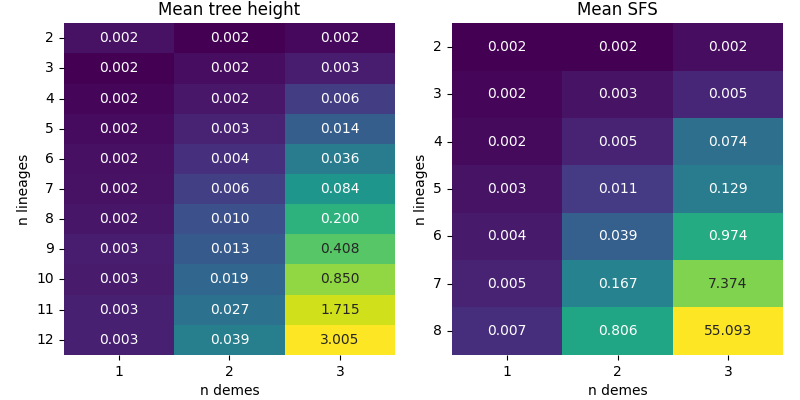
\includegraphics[width=\textwidth]{figures/executions_times}
    \caption{
        Total execution times in seconds for different numbers of lineages and demes.
        The different subplots consider the default and block-counting state spaces with one locus.
        Note that the computation of the SFS required $n$ independent matrix exponentiations, where $n$ is the number of lineages.
    }
    \label{fig:executions_times}
\end{figure}

